\documentclass[12pt]{article}

\usepackage{amsmath, mathtools}
\usepackage{amsfonts}
\usepackage{amssymb}
\usepackage{graphicx}
\usepackage{colortbl}
\usepackage{xr}
\usepackage{hyperref}
\usepackage{longtable}
\usepackage{xfrac}
\usepackage{tabularx}
\usepackage{float}
\usepackage{siunitx}
\usepackage{booktabs}
\usepackage{caption}
\usepackage{pdflscape}
\usepackage{afterpage}
\usepackage{placeins}
\usepackage[shortlabels]{enumitem}

\usepackage[round]{natbib}

%\usepackage{refcheck}

\hypersetup{
    bookmarks=true,         % show bookmarks bar?
    colorlinks=true,        % false: boxed links; true: colored links
    linkcolor=red,          % color of internal links (change box color with linkbordercolor)
    citecolor=green,        % color of links to bibliography
    filecolor=magenta,      % color of file links
    urlcolor=cyan           % color of external links
}

%% Comments

\usepackage{color}

\newif\ifcomments\commentstrue %displays comments
%\newif\ifcomments\commentsfalse %so that comments do not display

\ifcomments
\newcommand{\authornote}[3]{\textcolor{#1}{[#3 ---#2]}}
\newcommand{\todo}[1]{\textcolor{red}{[TODO: #1]}}
\else
\newcommand{\authornote}[3]{}
\newcommand{\todo}[1]{}
\fi

\newcommand{\wss}[1]{\authornote{blue}{SS}{#1}} 
\newcommand{\plt}[1]{\authornote{magenta}{TPLT}{#1}} %For explanation of the template
\newcommand{\an}[1]{\authornote{cyan}{Author}{#1}}

%% Common Parts

\newcommand{\progname}{Sayyara}
\newcommand{\authname}{Team 3, Tiny Coders
	\\ Arkin Modi
	\\ Joy Xiao
	\\ Leon So
	\\ Timothy Choy} % AUTHOR NAMES

\usepackage{hyperref}
\hypersetup{colorlinks=true, linkcolor=blue, citecolor=blue, filecolor=blue,
	urlcolor=blue, unicode=false}
\urlstyle{same}

\usepackage{parskip}
\usepackage{geometry}
\geometry{a4paper, portrait, margin=1in}


% For easy change of table widths
\newcommand{\colZwidth}{1.0\textwidth}
\newcommand{\colAwidth}{0.13\textwidth}
\newcommand{\colBwidth}{0.82\textwidth}
\newcommand{\colCwidth}{0.1\textwidth}
\newcommand{\colDwidth}{0.05\textwidth}
\newcommand{\colEwidth}{0.8\textwidth}
\newcommand{\colFwidth}{0.17\textwidth}
\newcommand{\colGwidth}{0.5\textwidth}
\newcommand{\colHwidth}{0.28\textwidth}

% Used so that cross-references have a meaningful prefix
\newcounter{defnum} %Definition Number
\newcommand{\dthedefnum}{GD\thedefnum}
\newcommand{\dref}[1]{GD\ref{#1}}
\newcounter{datadefnum} %Data definition Number
\newcommand{\ddthedatadefnum}{DD\thedatadefnum}
\newcommand{\ddref}[1]{DD\ref{#1}}
\newcounter{theorynum} %Theory Number
\newcommand{\tthetheorynum}{T\thetheorynum}
\newcommand{\tref}[1]{T\ref{#1}}
\newcounter{tablenum} %Table Number
\newcommand{\tbthetablenum}{T\thetablenum}
\newcommand{\tbref}[1]{TB\ref{#1}}
\newcounter{assumpnum} %Assumption Number
\newcommand{\atheassumpnum}{P\theassumpnum}
\newcommand{\aref}[1]{A\ref{#1}}
\newcounter{goalnum} %Goal Number
\newcommand{\gthegoalnum}{P\thegoalnum}
\newcommand{\gsref}[1]{GS\ref{#1}}
\newcounter{instnum} %Instance Number
\newcommand{\itheinstnum}{IM\theinstnum}
\newcommand{\iref}[1]{IM\ref{#1}}
\newcounter{reqnum} %Requirement Number
\newcommand{\rthereqnum}{P\thereqnum}
\newcommand{\rref}[1]{R\ref{#1}}
\newcounter{nfrnum} %NFR Number
\newcommand{\rthenfrnum}{NFR\thenfrnum}
\newcommand{\nfrref}[1]{NFR\ref{#1}}
\newcounter{lcnum} %Likely change number
\newcommand{\lthelcnum}{LC\thelcnum}
\newcommand{\lcref}[1]{LC\ref{#1}}

\usepackage{fullpage}

\newcommand{\deftheory}[9][Not Applicable]
{
\newpage
\noindent \rule{\textwidth}{0.5mm}

\paragraph{RefName: } \textbf{#2} \phantomsection 
\label{#2}

\paragraph{Label:} #3

\noindent \rule{\textwidth}{0.5mm}

\paragraph{Equation:}

#4

\paragraph{Description:}

#5

\paragraph{Notes:}

#6

\paragraph{Source:}

#7

\paragraph{Ref.\ By:}

#8

\paragraph{Preconditions for \hyperref[#2]{#2}:}
\label{#2_precond}

#9

\paragraph{Derivation for \hyperref[#2]{#2}:}
\label{#2_deriv}

#1

\noindent \rule{\textwidth}{0.5mm}

}

\begin{document}

\title{Software Requirements Specification for \progname: Progressive Web Application for Independent
	Automotive Repair Shop Industry}
\author{\authname}
\date{\today}

\maketitle

~\newpage

\pagenumbering{roman}

\tableofcontents

~\newpage

\begin{table}[hp]
	\caption{Revision History} \label{TblRevisionHistory}
	\begin{tabularx}{\textwidth}{llX}
		\toprule
		\textbf{Date}      & \textbf{Developer(s)} & \textbf{Change}                                                                    \\
		\midrule
		September 30, 2022 & Leon So               & Add purpose of project                                                             \\
		September 30, 2022 & Joy Xiao              & Add stakeholders                                                                   \\
		September 30, 2022 & Leon So               & Add functional requirements for authentication                                     \\
		September 30, 2022 & Arkin Modi            & Add open issues and new problems sections (effects on the current environment)     \\
		October 1, 2022    & Timothy Choy          & Add mandated constraints                                                           \\
		October 1, 2022    & Arkin Modi            & Add user documentation and training, waiting room and ideas for solutions sections \\
		October 1, 2022    & Arkin Modi            & Add project planning, migration to the new product, risks, and costs sections      \\
		October 2, 2022    & Leon So               & Add current situation and appointment diagram                                      \\
		October 2, 2022    & Joy Xiao              & Add current situation quote and invitation diagram                                 \\
		October 3, 2022    & Leon So               & Add current situation work order diagram                                           \\
		October 3, 2022    & Leon So               & Add functional requirements for employees management                               \\
		October 3, 2022    & Joy Xiao              & Add appointment FRs                                                                \\
		October 3, 2022    & Arkin Modi            & Add planning of the development phases and new problems sections                   \\
		October 3, 2022    & Arkin Modi            & Add off-the-shelf solutions sections                                               \\
		October 3, 2022    & Arkin Modi            & Add functional requirements for work orders                                        \\
		October 4, 2022    & Leon So               & Add context of work diagram                                                        \\
		October 4, 2022    & Leon So               & Add SRS subtitle                                                                   \\
		October 4, 2022    & Joy Xiao              & Add service functional requirements                                                \\
		October 4, 2022    & Arkin Modi            & Add functional requirements for quotes                                             \\
		October 4, 2022    & Joy Xiao              & Add non functional requirements                                                    \\
		October 5, 2022    & Leon So               & Add functional requirements for password reset                                     \\
		October 5, 2022    & Joy Xiao              & Add work partitioning                                                              \\
		\bottomrule
	\end{tabularx}
\end{table}

\newpage

\pagenumbering{arabic}

This document describes the requirements for Sayyara. The template for the Software Requirements
Specification (SRS) is a subset of the Volere template~\citep{RobertsonAndRobertson2012}. If you
make further modifications to the template, you should explicitly state what modifications were
made.

\section{Project Drivers}

\subsection{The Purpose of the Project}

Independent auto repair shops do not have an efficient way of reaching and interacting with new
customers. Currently, many independent shop owners rely on word-of-mouth referrals as a main
channel to acquiring new customers. Independent auto repair shops are also spending a significant
amount of their time on administrative work such as managing appointments and providing quotes. As
a result, independent auto repair shops have a difficult time competing with larger repair shops
which have dedicated systems and services in place.

On the other hand, customers do not have an effective way to find and compare auto repair shops.
Currently, one of the only ways to compare repair shops is by manually searching or reaching out to
repair shops one-by-one. This process can often be repetitive and time-consuming.

Sayyara is a progressive web application (PWA) which will act as a single platform for independent
auto repair shops and vehicle owners. This platform will allow independent auto repair shops and
vehicle owners to interact in a more efficient and effective manner. Vehicle owners can search for
auto repair shops and services based on a variety of search filters; request quotes for service;
book, view, and manage service appointments. On the application, auto repair shop owners will have
full shop management capabilities such as: adding and managing a list of employees; managing a list
of service types and corresponding service appointment availabilities; managing store information
such as location, hours of operation, and contact information. Auto repair shop owners and
employees will be able to manage quotes, service appointments, and work orders from a single
application. Ultimately, Sayyara will significantly improve the auto repair experience for both
independent auto repair shops and vehicle owners.

\subsection{The Stakeholders}

\subsubsection{The Client}
The client of the project is Nabeel Ibrahim. Nabeel will be the point of contact throughout the
development of the project.

\subsubsection{The Customers}
The customers of Sayyara will be independent auto repair shop owners, shop employees, and vehicle
owners who are looking for a vehicle repair or maintenance service.

\subsubsection{Other Stakeholders}
Other stakeholders of the project are the developers, Tiny Coders, who are designing and
implementing the project.

\subsection{Mandated Constraints}

\subsubsection{Solution Constraints}
\emph{Description:} The product shall be built as a Progressive Web Application (PWA)\\
\emph{Rationale:} The supervisor wants the application to be a PWA\\
\emph{Fit Criterion:} The product shall be written using the Next.js PWA plugin

\emph{Description:} The product shall be able to function on a variety of devices, such as on a computer, on tablets and on most modern phones\\
\emph{Rationale:} Users will be accessing this product in a variety of scenarios, and will have access to different devices\\
\emph{Fit Criterion:} The product shall be tested to function properly on Chrome's device toolbar, which includes the following devices:
\begin{itemize}
	\item iPhone SE
	\item iPhone XR
	\item iPhone 12 Pro
	\item Pixel 5
	\item Samsung Galaxy S8+
	\item Samsung Galaxy S20 Ultra
	\item iPad Air
	\item iPad Mini
	\item Surface Pro 7
	\item Surface Duo
	\item Galaxy Fold
	\item Samsung Galaxy A51/71
	\item Nest Hub
	\item Nest Hub Max
\end{itemize}
However, due to timing constraints, testing will only be run on the most popular cases, which would include the iPhone, Pixel and Samsung phones, as well as iPad and Galaxy tablets.

\subsubsection{Implementation Environment of the Current System}
In the current design of the product, the product shall be implemented in a cloud hosted serverless
environment. In this specific case, it shall be AWS Lambda. The product itself shall also be able
to function properly with any web browser and operating system.

\subsubsection{Partner or Collaborative Applications}
In the current design of the product, there are no partner or collaborative applications that will
work along with the product. Therefore, there are no partner or collaborative constraints.

\subsubsection{Off-the-Shelf Software}
The following off-the-shelf software will be utilized:
\begin{itemize}
	\item Next.js (and Next PWA)
\end{itemize}

\subsubsection{Anticipated Workplace Environment}
The anticipated workplace environment will be very broad. The product can be used from anywhere the
user has access to a device and internet to run the application.

\subsubsection{Schedule Constraints}
As stated in the SFWRENG 4G06 course outline, the schedule constraints are as follows:
\begin{table}[H]
	\centering
	\caption{Schedule Constraints}
	\vspace{5pt}
	\begin{tabular}{|p{0.3\textwidth}|p{0.6\textwidth}|}
		\hline
		\textbf{Date}   & \textbf{Deliverable}               \\
		\hline
		Oct 19, 2022    & Hazard Analysis                    \\
		\hline
		Nov 2, 2022     & Verification and Validation Plan   \\
		\hline
		Nov 14-25, 2022 & Proof of Concept Demo              \\
		\hline
		Jan 18, 2023    & Design Document                    \\
		\hline
		Feb 6-17, 2023  & Revision 0 Demo                    \\
		\hline
		Mar 8, 2023     & Verification and Validation Report \\
		\hline
		Mar 20-31, 2023 & Final Demo (Rev 1)                 \\
		\hline
		Apr 5, 2023     & Final Documentation                \\
		\hline
	\end{tabular}
\end{table}

\subsubsection{Budget Constraints}
The project has no monetary budget. If there are any necessary purchases for development, the cost
shall be paid by the project members and reimbursed by the supervisor. Furthermore, these purchases
may not exceed \$750.

\subsubsection{Enterprise Constraints}
The project will require authentication in the form of users logging in. The current implementation
of the project will require users to authenticate with a username and password. In the future, SSO
may be used.

\subsection{Naming Conventions and Terminology}

\subsection{Relevant Facts and Assumptions}

User characteristics should go under assumptions.

\section{Functional Requirements}

\subsection{The Scope of the Work and the Product}

\subsubsection{The Current Situation}
The current interactions between independent auto repair shop owners, employees, and customers
(i.e., vehicle owners), are often a manual process. Outlined below are models for interactions
between the independent auto repair shop owners, employees, customers, and the proposed system.
\begin{figure}[!hbp]
	\centering
	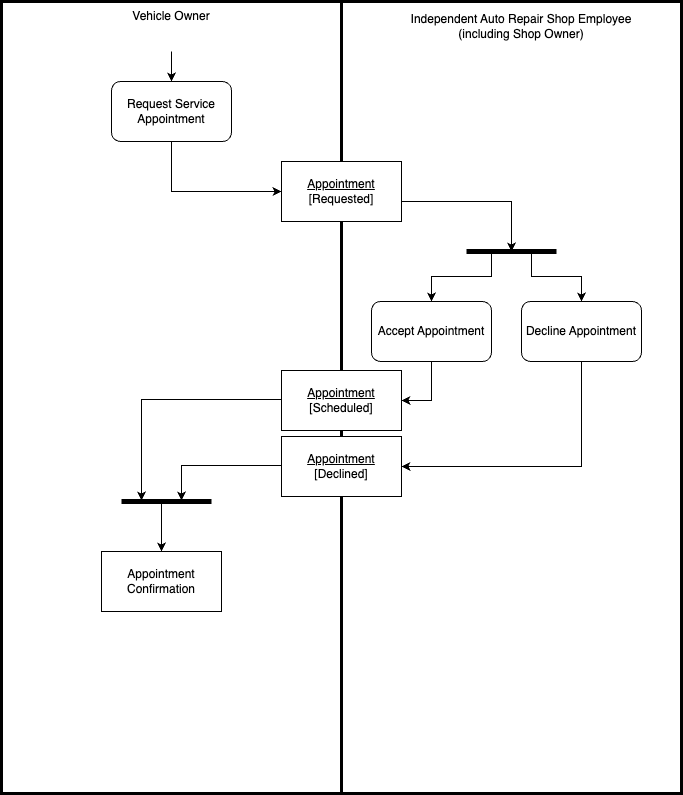
\includegraphics[width=\linewidth/2]{./diagrams/Appointments.png}
	\caption{Service Appointments}
\end{figure}
\FloatBarrier
\begin{figure}[!hbp]
	\centering
	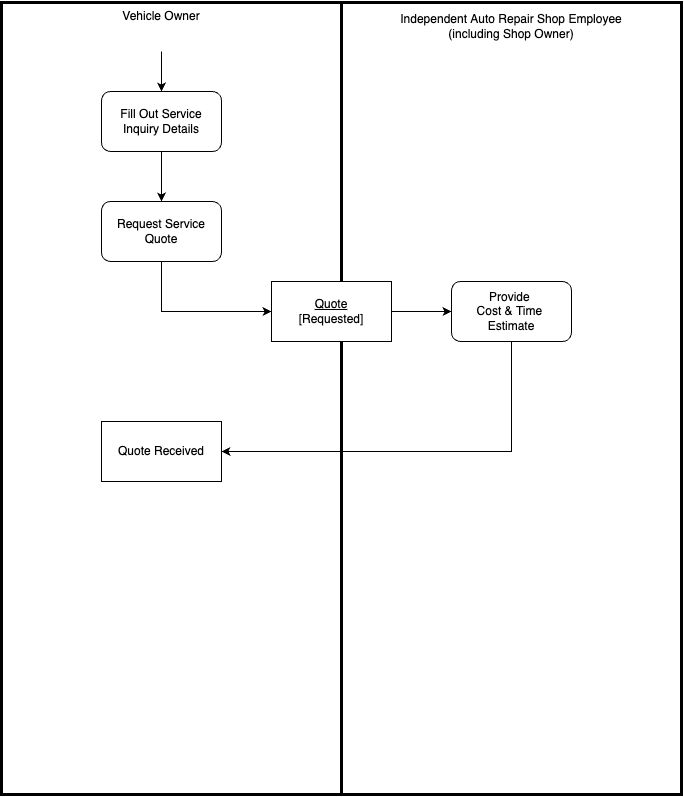
\includegraphics[width=\linewidth/2]{./diagrams/Quotes.png}
	\caption{Service Quotes}
\end{figure}
\FloatBarrier
\begin{figure}[!hbp]
	\centering
	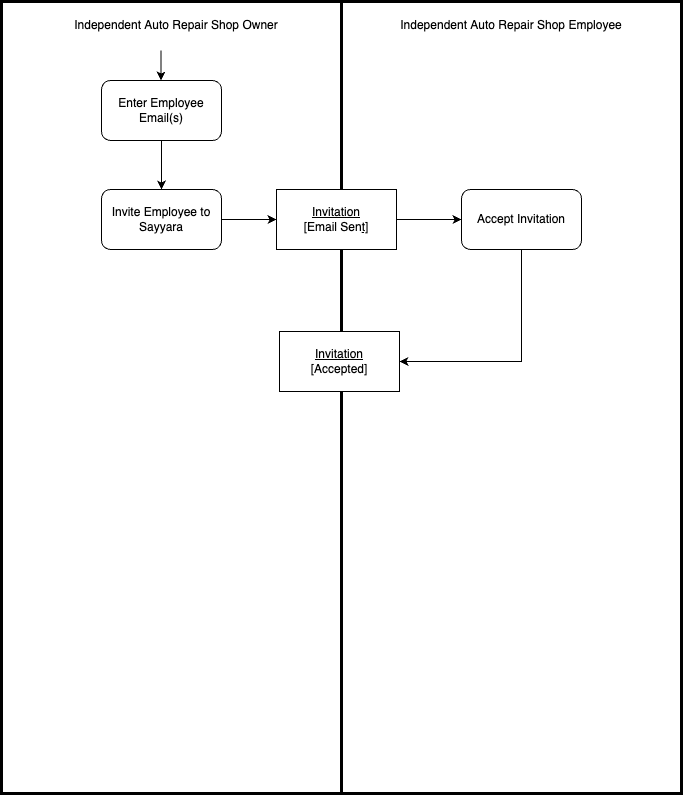
\includegraphics[width=\linewidth/2]{./diagrams/Invitation.png}
	\caption{Employee Invitation to Join Auto Repair Shop}
\end{figure}
\FloatBarrier
\begin{figure}[!hbp]
	\centering
	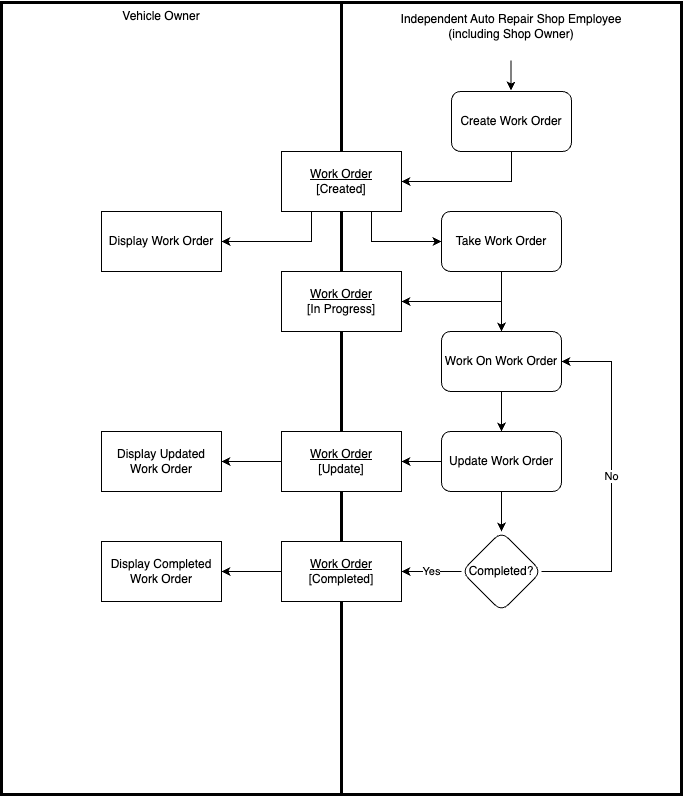
\includegraphics[width=\linewidth/2]{./diagrams/WorkOrder.png}
	\caption{Work Orders}
\end{figure}
\FloatBarrier

\subsubsection{Context of the Work}
The context diagram depicted below illustrates the interactions of the system with adjacent
external systems and services.
\begin{figure}[!hbp]
	\centering
	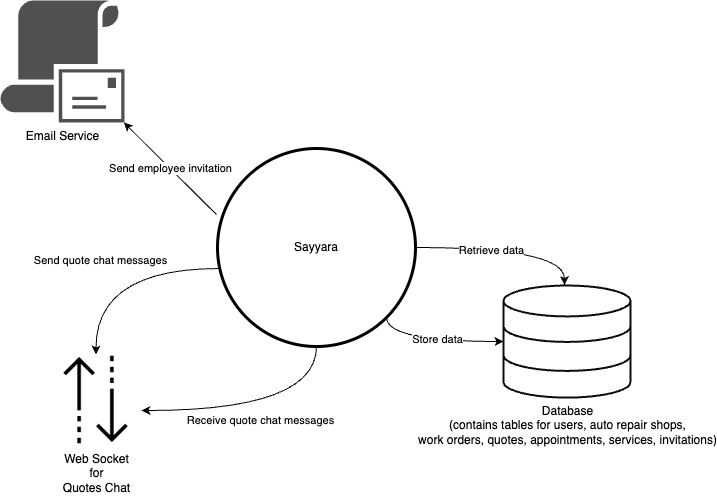
\includegraphics[width=\linewidth/2]{./diagrams/ContextOfWork.png}
	\caption{Context Diagram (Sayyara)}
\end{figure}
\FloatBarrier

\newpage
\subsubsection{Work Partitioning}
\begin{table}[H]
	\caption{Work Partitioning Events}
	\centering
	\begin{tabular}{|c|p{3.5cm}|c|p{3.5cm}|}
		\hline
		\textbf{Event Number} & \centering\textbf{Event Name}  & \textbf{Input} & \textbf{Output}    \\
		\hline
		1                     & Sign up for account            & User           & Database           \\
		\hline
		2                     & Login to account               & User           & Database           \\
		\hline
		3                     & Reset password                 & User           & Database           \\
		\hline
		4                     & Book appointment               & Database       & Database           \\
		\hline
		5                     & Edit appointment               & Database       & Database           \\
		\hline
		6                     & Cancel appointment             & Database       & Database           \\
		\hline
		7                     & Set appointment availability   & Database       & Database           \\
		\hline
		8                     & View past quotes               & User           & Database           \\
		\hline
		9                     & View quote details             & User           & Database           \\
		\hline
		10                    & Request a quote                & Web Socket     & Database           \\
		\hline
		11                    & Cancel quote request           & User           & Database           \\
		\hline
		12                    & Update quote request           & User           & Database/Websocket \\
		\hline
		13                    & Copy a quote request           & Database       & Database/Websocket \\
		\hline
		14                    & Respond to quote request       & Websocket      & Database           \\
		\hline
		15                    & Accept quote response          & Websocket      & Database           \\
		\hline
		16                    & Request additional information & Websocket      & Database           \\
		\hline
		17                    & Appointment scheduled          & User           & Database           \\
		\hline
		18                    & Appointment cancelled          & User           & Database           \\
		\hline
		19                    & Search for work order          & User           & Database           \\
		\hline
	\end{tabular}
\end{table}

\begin{table}[H]
	\caption{Work Partitioning Events Continued}
	\centering
	\begin{tabular}{|c|p{3.5cm}|c|p{3.5cm}|}
		\hline
		\textbf{Event Number} & \centering\textbf{Event Name}     & \textbf{Input} & \textbf{Output}        \\
		\hline
		20                    & View past work orders             & User           & Database               \\
		\hline
		21                    & Update work order                 & User           & Database               \\
		\hline
		22                    & Work order payment                & User           & Database/Email service \\
		\hline
		23                    & View work order details           & User           & Database               \\
		\hline
		24                    & Invite employee to shop           & User           & Database/Email service \\
		\hline
		25                    & Search for employee               & User           & Database               \\
		\hline
		26                    & View list of employees            & User           & Database               \\
		\hline
		27                    & Remove employee from shop         & User           & Database               \\
		\hline
		28                    & Add shop services to shop profile & User           & Database               \\
		\hline
		29                    & Search for service                & User           & Database               \\
		\hline
		30                    & Edit service type                 & User           & Database               \\
		\hline
		31                    & Delete service type               & User           & Database               \\
		\hline
	\end{tabular}
\end{table}

\subsubsection{Individual Product Use Cases}

\subsection{Functional Requirements}
\subsubsection{Authentication}
\begin{enumerate}[label=BE\arabic*., series=business_events]
	\item The user wants to sign up for an account
	      \begin{enumerate}[VP\arabic*.]
		      \item Viewpoint: Vehicle Owner
		            \begin{enumerate}
			            \item The system shall allow the user to enter an email and password
			            \item The system shall allow the user to enter their name
			            \item The system shall allow the user to enter their phone number
			            \item The system shall transition to the vehicle owner landing page after the registration process is
			                  complete and successful
			            \item The system shall allow the user to cancel and exit the registration process
		            \end{enumerate}

		      \item Viewpoint: Auto Repair Shop Owner
		            \begin{enumerate}
			            \item The system shall allow the user to enter an email and password
			            \item The system shall allow the user to enter their name
			            \item The system shall allow the user to enter their phone number
			            \item The system shall allow the user to enter the shop name
			            \item The system shall allow the user to enter the shop address
			            \item The system shall allow the user to enter the shop phone number
			            \item The system shall transition to the shop owner landing page after the registration process is
			                  complete and successful
			            \item The system shall allow the user to cancel and exit the registration process
		            \end{enumerate}

		      \item Viewpoint: Auto Repair Shop Employee
		            \begin{enumerate}
			            \item The system shall allow the user to enter an email and password
			            \item The system shall allow the user to enter their name
			            \item The system shall allow the user to enter their phone number
			            \item The system shall transition to the employee landing page after the registration process is complete
			                  and successful
			            \item The system shall allow the user to cancel and exit the registration process
		            \end{enumerate}
	      \end{enumerate}

	\item The user wants to login to their account
	      \begin{enumerate}[VP\arabic*.]
		      \item Viewpoint: Vehicle Owner
		            \begin{enumerate}
			            \item The system shall allow the user to enter their email and password
			            \item The system shall transition to the vehicle owner landing page after the login process is complete
			                  and successful
			            \item The system shall allow the user to cancel and exit the login process
		            \end{enumerate}

		      \item Viewpoint: Auto Repair Shop Owner
		            \begin{enumerate}
			            \item The system shall allow the user to enter their email and password
			            \item The system shall transition to the shop owner landing page after the login process is complete and
			                  successful
			            \item The system shall allow the user to cancel and exit the login process
		            \end{enumerate}

		      \item Viewpoint: Auto Repair Shop Employee
		            \begin{enumerate}
			            \item The system shall allow the user to enter their email and password
			            \item The system shall transition to the employee landing page after the login process is complete and
			                  successful
			            \item The system shall allow the user to cancel and exit the login process
		            \end{enumerate}
	      \end{enumerate}

	\item The user wants to reset their password
	      \begin{enumerate}[VP\arabic*.]
		      \item Viewpoint: Vehicle Owner
		            \begin{enumerate}
			            \item The system shall allow the user to enter their email
			            \item The system shall send a password reset code to the email if the email is associated with an account
			            \item The system shall display a countdown for the password reset code expiration
			            \item The system shall ask the user for a new password if the code matches
		            \end{enumerate}

		      \item Viewpoint: Auto Repair Shop Owner
		            \begin{enumerate}
			            \item The system shall allow the user to enter their email
			            \item The system shall send a password reset code to the email if the email is associated with an account
			            \item The system shall display a countdown for the password reset code expiration
			            \item The system shall ask the user for a new password if the code matches
		            \end{enumerate}

		      \item Viewpoint: Auto Repair Shop Employee
		            \begin{enumerate}
			            \item The system shall allow the user to enter their email
			            \item The system shall send a password reset code to the email if the email is associated with an account
			            \item The system shall display a countdown for the password reset code expiration
			            \item The system shall ask the user for a new password if the code matches
		            \end{enumerate}
	      \end{enumerate}
\end{enumerate}

\subsubsection{Appointments}
\begin{enumerate}[resume*=business_events]
	\item The user wants to book an appointment
	      \begin{enumerate}[VP\arabic*.]
		      \item Viewpoint: Vehicle Owner
		            \begin{enumerate}
			            \item The system shall populate the service request information from the quote
			            \item The system shall populate the service request information from the if a canned job is selected
			            \item The system shall allow the user to filter available appointments times
			            \item The system shall display dates and times where appointments are available
			            \item The system shall allow the user to select an appointment time slot to book
			            \item The system shall allow the user to sync the appointment time to their calendar
			            \item The system shall transition to the view appointments page
			            \item The system shall allow the user to cancel and exit the appointment process
		            \end{enumerate}
		      \item Viewpoint: Auto Repair Shop Owner
		            \begin{enumerate}
			            \item The system shall allow the user to enter a name
			            \item The system shall allow the user to enter a phone number
			            \item The system shall allow the user to enter service details
			            \item The system shall allow the user to select an available time slot
			            \item The system shall transition to the view appointments page
			            \item The system shall allow the user to cancel and exit the appointment process
		            \end{enumerate}
		      \item Viewpoint: Auto Repair Shop Employee
		            \begin{enumerate}
			            \item The system shall allow the user to enter a name
			            \item The system shall allow the user to enter a phone number
			            \item The system shall allow the user to enter service details
			            \item The system shall allow the user to select an available time slot
			            \item The system shall transition to the view appointments page
			            \item The system shall allow the user to cancel and exit the appointment process
		            \end{enumerate}
	      \end{enumerate}

	\item The user wants to edit an appointment
	      \begin{enumerate}[VP\arabic*.]
		      \item Viewpoint: Vehicle Owner
		            \begin{enumerate}
			            \item The system shall allow the user to select a scheduled appointment
			            \item The system shall allow the user to select another available timeslot
		            \end{enumerate}
		      \item Viewpoint: Auto Repair Shop Owner
		            \begin{enumerate}
			            \item The system shall allow the user to select a scheduled appointment
			            \item The system shall allow the user to update service details
			            \item The system shall allow the user to select another available timeslot
		            \end{enumerate}
		      \item Viewpoint: Auto Repair Shop Employee
		            \begin{enumerate}
			            \item The system shall allow the user to select a scheduled appointment
			            \item The system shall allow the user to update service details
			            \item The system shall allow the user to select another available timeslot
		            \end{enumerate}
	      \end{enumerate}

	\item The user wants to cancel an appointment
	      \begin{enumerate}[VP\arabic*.]
		      \item Viewpoint: Vehicle Owner
		            \begin{enumerate}
			            \item The system shall allow the user to select a scheduled appointment
			            \item The system shall allow the user to cancel the appointment
		            \end{enumerate}
		      \item Viewpoint: Auto Repair Shop Owner
		            \begin{enumerate}
			            \item The system shall allow the user to select a scheduled appointment
			            \item The system shall allow the user to cancel the appointment
		            \end{enumerate}
		      \item Viewpoint: Auto Repair Shop Employee
		            \begin{enumerate}
			            \item The system shall allow the user to select a scheduled appointment
			            \item The system shall allow the user to cancel the appointment
		            \end{enumerate}
	      \end{enumerate}

	\item The user wants to set appointment availability
	      \begin{enumerate}[VP\arabic*.]
		      \item Viewpoint: Vehicle Owner
		            \begin{enumerate}
			            \item[] N/A
		            \end{enumerate}
		      \item Viewpoint: Auto Repair Shop Owner
		            \begin{enumerate}
			            \item The system shall allow the user to set the days that appointments can be made
			            \item The system shall allow the user to set the hours that appointments can be made
			            \item The system shall allow the user to set the number of appointments that can be booked every hour
		            \end{enumerate}
		      \item Viewpoint: Auto Repair Shop Employee
		            \begin{enumerate}
			            \item[] N/A
		            \end{enumerate}
	      \end{enumerate}
\end{enumerate}

\subsubsection{Quotes}
\begin{enumerate}[resume*=business_events]
	\item The user wants view past quotes
	      \begin{enumerate}[VP\arabic*.]
		      \item Viewpoint: Vehicle Owner
		            \begin{enumerate}
			            \item The system shall list all quotes
		            \end{enumerate}
		      \item Viewpoint: Auto Repair Shop Owner
		            \begin{enumerate}
			            \item The system shall allow the user to enter the quote ID, customer phone number, and customer name
			            \item The system shall list all quotes matching the inputted criteria
		            \end{enumerate}
		      \item Viewpoint: Auto Repair Shop Employee
		            \begin{enumerate}
			            \item The system shall allow the user to enter the quote ID, customer phone number, and customer name
			            \item The system shall list all quotes matching the inputted criteria
		            \end{enumerate}
	      \end{enumerate}

	\item The user wants view details about a quote
	      \begin{enumerate}[VP\arabic*.]
		      \item Viewpoint: Vehicle Owner
		            \begin{enumerate}
			            \item The system shall allow the user to view the car details, contact details, desired services,
			                  replacement parts condition and source, extra notes, file attachments and time availability from
			                  the quote request
			            \item The system shall allow the user to view the estimated price, a list of services, the estimated
			                  time, a list of required parts, and discounts from the quote response
		            \end{enumerate}
		      \item Viewpoint: Auto Repair Shop Owner
		            \begin{enumerate}
			            \item The system shall allow the user to view the car details, contact details, desired services,
			                  replacement parts condition and source, extra notes, file attachments and time availability from
			                  the quote request
			            \item The system shall allow the user to view the estimated price, a list of services, the estimated
			                  time, a list of required parts, and discounts from the quote response
		            \end{enumerate}
		      \item Viewpoint: Auto Repair Shop Employee
		            \begin{enumerate}
			            \item The system shall allow the user to view the car details, contact details, desired services,
			                  replacement parts condition and source, extra notes, file attachments and time availability from
			                  the quote request
			            \item The system shall allow the user to view the estimated price, a list of services, the estimated
			                  time, a list of required parts, and discounts from the quote response
		            \end{enumerate}
	      \end{enumerate}
\end{enumerate}

\begin{enumerate}[resume*=business_events]
	\item The user wants to request a quote
	      \begin{enumerate}[VP\arabic*.]
		      \item Viewpoint: Vehicle Owner
		            \begin{enumerate}
			            \item The system shall automatically populate car details and contact details if present in the user's
			                  profile
			            \item The system shall allow the user to enter their car details, contact details, desired services,
			                  replacement parts condition and source, extra notes, file attachments and time availability
			            \item The system shall confirm to the user that the request has been submitted
			            \item The system shall generate a quote ID and assign it to the newly created quote
		            \end{enumerate}
		      \item Viewpoint: Auto Repair Shop Owner
		            \begin{enumerate}
			            \item The system shall notify the user of the newly created quote request by the vehicle owner
		            \end{enumerate}
		      \item Viewpoint: Auto Repair Shop Employee
		            \begin{enumerate}
			            \item The system shall notify the user of the newly created quote request by the vehicle owner
		            \end{enumerate}
	      \end{enumerate}

	\item The user wants cancel a quote request
	      \begin{enumerate}[VP\arabic*.]
		      \item Viewpoint: Vehicle Owner
		            \begin{enumerate}
			            \item The system shall list active quotes
			            \item The system shall allow the user to cancel a quote
		            \end{enumerate}
		      \item Viewpoint: Auto Repair Shop Owner
		            \begin{enumerate}
			            \item[] N/A
		            \end{enumerate}
		      \item Viewpoint: Auto Repair Shop Employee
		            \begin{enumerate}
			            \item[] N/A
		            \end{enumerate}
	      \end{enumerate}

	\item The user wants update a quote request
	      \begin{enumerate}[VP\arabic*.]
		      \item Viewpoint: Vehicle Owner
		            \begin{enumerate}
			            \item The system shall list active quotes
			            \item The system shall allow the user to update a quote
		            \end{enumerate}
		      \item Viewpoint: Auto Repair Shop Owner
		            \begin{enumerate}
			            \item The system shall notify the user of the updated quote request
		            \end{enumerate}
		      \item Viewpoint: Auto Repair Shop Employee
		            \begin{enumerate}
			            \item The system shall notify the user of the updated quote request
		            \end{enumerate}
	      \end{enumerate}

	\item The user wants to copy an existing quote request
	      \begin{enumerate}[VP\arabic*.]
		      \item Viewpoint: Vehicle Owner
		            \begin{enumerate}
			            \item The system shall allow the user to create a new quote request using the data from an existing quote
			                  request
		            \end{enumerate}
		      \item Viewpoint: Auto Repair Shop Owner
		            \begin{enumerate}
			            \item[] N/A
		            \end{enumerate}
		      \item Viewpoint: Auto Repair Shop Employee
		            \begin{enumerate}
			            \item[] N/A
		            \end{enumerate}
	      \end{enumerate}

	\item The user wants to respond to a quote request
	      \begin{enumerate}[VP\arabic*.]
		      \item Viewpoint: Vehicle Owner
		            \begin{enumerate}
			            \item The system shall notify the user of the quote response from the automotive repair shop
		            \end{enumerate}
		      \item Viewpoint: Auto Repair Shop Owner
		            \begin{enumerate}
			            \item The system shall allow the user to enter the estimated price, a list of services, the estimated
			                  time, a list of required parts, and discounts
			            \item The system shall automatically apply local taxes
			            \item The system shall send the quote to the customer
			            \item The system shall send a notification to the customer
		            \end{enumerate}
		      \item Viewpoint: Auto Repair Shop Employee
		            \begin{enumerate}
			            \item The system shall allow the user to enter the estimated price, a list of services, the estimated
			                  time, a list of required parts, and discounts
			            \item The system shall automatically apply local taxes
			            \item The system shall send the quote to the customer
			            \item The system shall send a notification to the customer
		            \end{enumerate}
	      \end{enumerate}

	\item The user would like to accept a quote response
	      \begin{enumerate}[VP\arabic*.]
		      \item Viewpoint: Vehicle Owner
		            \begin{enumerate}
			            \item The system shall allow the user to accept a quote response
			            \item The system shall navigate the user to the appointment booking process
		            \end{enumerate}
		      \item Viewpoint: Auto Repair Shop Owner
		            \begin{enumerate}
			            \item[] N/A
		            \end{enumerate}
		      \item Viewpoint: Auto Repair Shop Employee
		            \begin{enumerate}
			            \item[] N/A
		            \end{enumerate}
	      \end{enumerate}

	\item The user would like to request additional information
	      \begin{enumerate}[VP\arabic*.]
		      \item Viewpoint: Vehicle Owner
		            \begin{enumerate}
			            \item The system shall allow the user to send messages to the automotive repair shop
			            \item The system shall allow the user to receive messages from the automotive repair shop
		            \end{enumerate}
		      \item Viewpoint: Auto Repair Shop Owner
		            \begin{enumerate}
			            \item The system shall allow the user to send messages to the customer
			            \item The system shall allow the user to receive messages from the customer
		            \end{enumerate}
		      \item Viewpoint: Auto Repair Shop Employee
		            \begin{enumerate}
			            \item The system shall allow the user to send messages to the customer
			            \item The system shall allow the user to receive messages from the customer
		            \end{enumerate}
	      \end{enumerate}
\end{enumerate}

\subsubsection{Work Orders}
\begin{enumerate}[resume*=business_events]
	\item An appointment has been scheduled
	      \begin{enumerate}[VP\arabic*.]
		      \item Viewpoint: Vehicle Owner
		            \begin{enumerate}
			            \item[] N/A
		            \end{enumerate}
		      \item Viewpoint: Auto Repair Shop Owner
		            \begin{enumerate}
			            \item The system shall create a work order
			            \item The system shall populate the customer data and vehicle data from the quote
			            \item The system shall populate the customer data and vehicle data from the appointment if the quote is
			                  not available
			            \item The system shall populate expected services performed and parts needed from the quote
			            \item The system shall populate expected services performed and parts needed from the appointment if the
			                  quote not available
		            \end{enumerate}
		      \item Viewpoint: Auto Repair Shop Employee
		            \begin{enumerate}
			            \item The system shall create a work order
			            \item The system shall populate the customer data and vehicle data from the quote
			            \item The system shall populate the customer data and vehicle data from the appointment if the quote is
			                  not available
			            \item The system shall populate expected services performed and parts needed from the quote
			            \item The system shall populate expected services performed and parts needed from the appointment if the
			                  quote not available
		            \end{enumerate}
	      \end{enumerate}

	\item An appointment has been cancelled
	      \begin{enumerate}[VP\arabic*.]
		      \item Viewpoint: Vehicle Owner
		            \begin{enumerate}
			            \item[] N/A
		            \end{enumerate}
		      \item Viewpoint: Auto Repair Shop Owner
		            \begin{enumerate}
			            \item The system shall delete the associated work order
		            \end{enumerate}
		      \item Viewpoint: Auto Repair Shop Employee
		            \begin{enumerate}
			            \item The system shall delete the associated work order
		            \end{enumerate}
	      \end{enumerate}

	\item The user wants to search for a work order
	      \begin{enumerate}[VP\arabic*.]
		      \item Viewpoint: Vehicle Owner
		            \begin{enumerate}
			            \item[] N/A
		            \end{enumerate}
		      \item Viewpoint: Auto Repair Shop Owner
		            \begin{enumerate}
			            \item The system shall allow the user to enter the customer name, assigned employee, service type, and a
			                  date range
			            \item The system shall list the work order matching the inputted criteria
		            \end{enumerate}
		      \item Viewpoint: Auto Repair Shop Employee
		            \begin{enumerate}
			            \item The system shall allow the user to enter the customer name, assigned employee, service type, and a
			                  date range
			            \item The system shall list the work order matching the inputted criteria
		            \end{enumerate}
	      \end{enumerate}

	\item The user wants to view past work orders
	      \begin{enumerate}[VP\arabic*.]
		      \item Viewpoint: Vehicle Owner
		            \begin{enumerate}
			            \item[] N/A
		            \end{enumerate}
		      \item Viewpoint: Auto Repair Shop Owner
		            \begin{enumerate}
			            \item The system shall list the past work orders
		            \end{enumerate}
		      \item Viewpoint: Auto Repair Shop Employee
		            \begin{enumerate}
			            \item The system shall list the past work orders
		            \end{enumerate}
	      \end{enumerate}

	\item The user wants update an work order
	      \begin{enumerate}[VP\arabic*.]
		      \item Viewpoint: Vehicle Owner
		            \begin{enumerate}
			            \item[] N/A
		            \end{enumerate}
		      \item Viewpoint: Auto Repair Shop Owner
		            \begin{enumerate}
			            \item The system shall list the open work orders
			            \item The system shall allow the user to edit the services performed, parts required, odometer readings,
			                  customer details, employee assigned, car details, discounts, digital vehicle inspection, and extra
			                  notes
			            \item The system shall update the work order with the entered values
		            \end{enumerate}
		      \item Viewpoint: Auto Repair Shop Employee
		            \begin{enumerate}
			            \item The system shall list the open work orders
			            \item The system shall allow the user to edit the services performed, parts required, odometer readings,
			                  customer details, employee assigned, car details, discounts, digital vehicle inspection, and extra
			                  notes
			            \item The system shall update the work order with the entered values
		            \end{enumerate}
	      \end{enumerate}

	\item The customer has paid for the work done on their vehicle
	      \begin{enumerate}[VP\arabic*.]
		      \item Viewpoint: Vehicle Owner
		            \begin{enumerate}
			            \item[] N/A
		            \end{enumerate}
		      \item Viewpoint: Auto Repair Shop Owner
		            \begin{enumerate}
			            \item The system shall send a copy of the work order to the assigned customer's email
			            \item The system shall mark the work order as ``Completed''
			            \item The system shall mark the associated appointment as ``Completed''
		            \end{enumerate}
		      \item Viewpoint: Auto Repair Shop Employee
		            \begin{enumerate}
			            \item The system shall send a copy of the work order to the assigned customer's email
			            \item The system shall mark the work order as ``Completed''
			            \item The system shall mark the associated appointment as ``Completed''
		            \end{enumerate}
	      \end{enumerate}

	\item The user wants to view the details of a work order
	      \begin{enumerate}[VP\arabic*.]
		      \item Viewpoint: Vehicle Owner
		            \begin{enumerate}
			            \item[] N/A
		            \end{enumerate}
		      \item Viewpoint: Auto Repair Shop Owner
		            \begin{enumerate}
			            \item The system shall list the shop details, services to be performed with their individual bill rates
			                  and expected number of hours for completion, parts required and their cost, odometer reading before
			                  and after service, customer details, assigned employee, car details, any applied discounts, final
			                  balance for the customer, warranty information, digital vehicle inspection, and any extra notes
		            \end{enumerate}
		      \item Viewpoint: Auto Repair Shop Employee
		            \begin{enumerate}
			            \item The system shall list the shop details, services to be performed with their individual bill rates
			                  and expected number of hours for completion, parts required and their cost, odometer reading before
			                  and after service, customer details, assigned employee, car details, any applied discounts, final
			                  balance for the customer, warranty information, digital vehicle inspection, and any extra notes
		            \end{enumerate}
	      \end{enumerate}

\end{enumerate}

\subsubsection{Employee Management}
\begin{enumerate}[resume*=business_events]
	\item The shop owner wants to invite an employee to their shop
	      \begin{enumerate}[VP\arabic*.]
		      \item Viewpoint: Vehicle Owner
		            \begin{enumerate}
			            \item[] N/A
		            \end{enumerate}
		      \item Viewpoint: Auto Repair Shop Owner
		            \begin{enumerate}
			            \item The system shall allow the user to enter employee email(s) to invite
			            \item The system shall send an invitation email to the invited employee(s)
		            \end{enumerate}
		      \item Viewpoint: Auto Repair Shop Employee
		            \begin{enumerate}
			            \item The system shall allow the user to accept an invitation
		            \end{enumerate}
	      \end{enumerate}

	\item The shop owner wants to search for an employee
	      \begin{enumerate}[VP\arabic*.]
		      \item Viewpoint: Vehicle Owner
		            \begin{enumerate}
			            \item[] N/A
		            \end{enumerate}
		      \item Viewpoint: Auto Repair Shop Owner
		            \begin{enumerate}
			            \item The system shall allow the user to enter search text to search for an employee
			            \item The system shall display a list of employees whose name or email matches the search text
		            \end{enumerate}
		      \item Viewpoint: Auto Repair Shop Employee
		            \begin{enumerate}
			            \item[] N/A
		            \end{enumerate}
	      \end{enumerate}

	\item The shop owner wants to view the list of employees
	      \begin{enumerate}[VP\arabic*.]
		      \item Viewpoint: Vehicle Owner
		            \begin{enumerate}
			            \item[] N/A
		            \end{enumerate}
		      \item Viewpoint: Auto Repair Shop Owner
		            \begin{enumerate}
			            \item The system shall display a list of employees
		            \end{enumerate}
		      \item Viewpoint: Auto Repair Shop Employee
		            \begin{enumerate}
			            \item[] N/A
		            \end{enumerate}
	      \end{enumerate}

	\item The shop owner wants to remove an employee
	      \begin{enumerate}[VP\arabic*.]
		      \item Viewpoint: Vehicle Owner
		            \begin{enumerate}
			            \item[] N/A
		            \end{enumerate}
		      \item Viewpoint: Auto Repair Shop Owner
		            \begin{enumerate}
			            \item The system shall allow the user to remove an employee
			            \item The system shall revoke the removed employee's access to the auto repair shop employee controls
		            \end{enumerate}
		      \item Viewpoint: Auto Repair Shop Employee
		            \begin{enumerate}
			            \item The system shall revoke the removed employee's access to the auto repair shop employee controls
		            \end{enumerate}
	      \end{enumerate}
\end{enumerate}

\subsubsection{Services}
\begin{enumerate}[resume*=business_events]
	\item The user wants to add available auto shop services to the shop profile
	      \begin{enumerate}[VP\arabic*.]
		      \item Viewpoint: Vehicle Owner
		            \begin{enumerate}
			            \item[] N/A
		            \end{enumerate}
		      \item Viewpoint: Auto Repair Shop Owner
		            \begin{enumerate}
			            \item The system shall allow the user to enter the name of the service
			            \item The system shall allow the user to enter a description for the service
			            \item The system shall allow the user to enter the estimated time for the service
			            \item The system shall allow the user to enter the parts used for the service including quantity,
			                  condition (new or used), build (OEM or aftermarket), and cost per part (before tax cost)
			            \item The system shall allow the user to enter the total price for the service (before tax price)
		            \end{enumerate}
		      \item Viewpoint: Auto Repair Shop Employee
		            \begin{enumerate}
			            \item[] N/A
		            \end{enumerate}
	      \end{enumerate}

	\item The user wants to search for auto repair or maintenance services
	      \begin{enumerate}[VP\arabic*.]
		      \item Viewpoint: Vehicle Owner
		            \begin{enumerate}
			            \item The system shall display the service details
		            \end{enumerate}
		      \item Viewpoint: Auto Repair Shop Owner
		            \begin{enumerate}
			            \item The system shall display the service details
			            \item The system shall allow the user to search for a specific service type
		            \end{enumerate}
		      \item Viewpoint: Auto Repair Shop Employee
		            \begin{enumerate}
			            \item The system shall display the service details
			            \item The system shall allow the user to search for a specific service type
		            \end{enumerate}
	      \end{enumerate}

	\item The user wants to edit a service type
	      \begin{enumerate}[VP\arabic*.]
		      \item Viewpoint: Vehicle Owner
		            \begin{enumerate}
			            \item[] N/A
		            \end{enumerate}
		      \item Viewpoint: Auto Repair Shop Owner
		            \begin{enumerate}
			            \item The system shall allow the user to update the details of a particular service
		            \end{enumerate}
		      \item Viewpoint: Auto Repair Shop Employee
		            \begin{enumerate}
			            \item[] N/A
		            \end{enumerate}
	      \end{enumerate}

	\item The user wants to delete a service type
	      \begin{enumerate}[VP\arabic*.]
		      \item Viewpoint: Vehicle Owner
		            \begin{enumerate}
			            \item[] N/A
		            \end{enumerate}
		      \item Viewpoint: Auto Repair Shop Owner
		            \begin{enumerate}
			            \item The system shall allow the user to delete the service from their shop page
		            \end{enumerate}
		      \item Viewpoint: Auto Repair Shop Employee
		            \begin{enumerate}
			            \item[] N/A
		            \end{enumerate}
	      \end{enumerate}
\end{enumerate}

\section{Non-functional Requirements}

\subsection{Look and Feel Requirements}
\begin{enumerate}[LF\arabic*.]
	\item The system shall adjust and scale to fit the physical screen size
	\item The system shall have fonts and colours that will allow users to easily read the text
	\item The system shall display dollar amounts rounded to 2 decimal places
\end{enumerate}

\subsection{Usability and Humanity Requirements}
\begin{enumerate}[UH\arabic*.]
	\item The system shall accessible by any desktop or mobile device and any operating system
	\item The system shall be accessible through the web browser and when the device is connected to internet
\end{enumerate}

\subsection{Performance Requirements}
\begin{enumerate}[PR\arabic*.]
	\item The system shall respond to the user's interactions within 0.5 seconds
\end{enumerate}

\subsection{Operational and Environmental Requirements}
\begin{enumerate}[OE\arabic*.]
	\item The system shall be able to operate on desktops and mobile devices
\end{enumerate}

\subsection{Maintainability and Support Requirements}
\begin{enumerate}[MS\arabic*.]
	\item The system shall be well documented
\end{enumerate}

\subsection{Security Requirements}
\begin{enumerate}[SR\arabic*.]
	\item The system shall keep user's data private
	\item The system shall limit the data shown to user's on a needs to know basis
\end{enumerate}

\subsection{Cultural Requirements}
\begin{enumerate}[CR\arabic*.]
	\item The system shall not use any text or images that will offend anyone that will use it
	\item The system will use Canadian English
\end{enumerate}

\subsection{Legal Requirements}
\begin{enumerate}[LR\arabic*.]
	\item The system shall not contain any assets which infringe on copyright claims
\end{enumerate}

\subsection{Health and Safety Requirements}
N/A

\section{Project Issues}

\subsection{Open Issues}

There are currently no known open issues that may lead to significant change to the product or its
design.

\subsection{Off-the-Shelf Solutions}

\subsubsection{Ready-Made Products}

There are existing services that solve many of the problems that this application aims to address.
These include AutoLeap (https://autoleap.com), Sayaaraa (https://sayaaraa.com), and KUKUI
(https://www.kukui.com). These are all paid services and most offer a trial period. Additional,
these app only address the shop management aspect of the problem. Openbay (https://app.openbay.com)
is an existing application that focuses on vehicle owner's needs. This application exclusively
operates in the United States of America.

\subsubsection{Resuable Components}

There are many libraries and frameworks available that can be reused to accelerate the building
process of the application. Next.js can be used to provide a framework to build the application.
Next.js comes with many out-of-box solutions for common website development problems. NextAuth.js
is a library designed to help simplify the authentication process. Prisma is a library designed to
help simplify the communication between the application and the database. Next-PWA is a library
designed to quickly bootstrap a Next.js application into a progressive web application.

A runtime and ecosystem that is available to use is Node.js. This runtime comes with a large
ecosystem of packages that can be reused and leveraged for common application components, including
the libraries listed previously.

All components listed above are free to use for private and commercial use.

\subsubsection{Products That Can Be Copied}

There are no known products available that can be legally copied for use in this application.

\subsection{New Problems}

\subsubsection{Effects on the Current Environment}

This application will change the way certain processes are preformed and these changes will impact
the users.

\textbf{Work Orders}

The work order system will affect the way automotive mechanics document their work. The data will
be inputted into the application therefore any failures can result in data loss.

\textbf{Appointments}

The appointments system will affect the way that both the customers and the employees schedule
appointments. The application will track daily appointment schedules and report time conflicts. The
application shall not lock the employee out of overriding the schedule.

\textbf{Quotes}

The quotes system will affect the way that both the customers and automotive repair shops
communicate in the service quotation process. The quotes will now be communicated partially or
completely through the application instead of completely in-person. Failure in this system may lead
to a loss in data.

\subsubsection{Effects on the Installed Systems}

The application will be completely stand alone and will not be interfacing with any existing
systems. The existing system may continue to coexist with the application at the user's discretion.

\subsubsection{Potential User Problems}

Any potential adverse reactions related to using the device in which application is being launched
on (e.g., computer, mobile device, tablet, etc.) would extend to the use of this application. The
application will not introduce any new adverse reactions to the user.

\subsubsection{Limitations in the Anticipated Implementation Environment That May Inhibit the New Product}

The database is not able to sustain the number of connections to serve all requests.

\subsubsection{Follow-Up Problems}

Any failures or downtime of third-party integrations may impact the overall availability and
operation of the application. These integrations include the database service provider, the email
server, and websocket provider. Additionally, this application will be dealing with user data. As
privacy laws around the world are getting stricter, there is a possibility application violates
these future laws that do not currently exist.

\subsection{Tasks}
\subsubsection{Project Planning}
The project schedule will follow the deadline for the deliverables outlined in the SFWRENG 4G06
course outline.

\begin{table}[H]
	\centering
	\caption{Project Tasks}
	\vspace{5pt}
	\begin{tabular}{|p{0.2\textwidth}|p{0.4\textwidth}|p{0.3\textwidth}|}
		\hline
		\textbf{Phase} & \textbf{Task}                      & \textbf{Due Date}                 \\
		\hline
		Phase 1        & Hazard Analysis                    & October 19, 2022                  \\
		\cline{2-3}    & Verification and Validation Plan   & November 2, 2022                  \\
		\cline{2-3}    & Proof of Concept Demonstration     & November 14, 2022                 \\
		\cline{2-3}    & Design Documentation               & January 18, 2023                  \\
		\cline{2-3}    & Revision 0 Demonstration           & February 6 \textemdash{} 17, 2023 \\
		\hline
		Phase 2        & Verification and Validation Report & March 8, 2023                     \\
		\cline{2-3}    & Final Demonstration                & March 20 \textemdash{} 31, 2023   \\
		\cline{2-3}    & Final Documentation                & April 5, 2023                     \\
		\hline
	\end{tabular}

	\label{project_tasks}
\end{table}

\subsubsection{Planning of the Development Phases}

The development of the project will be conducted in two phases:

\begin{enumerate}
	\item Initial development of application and documentation
	\item Refinement of application and documentation
\end{enumerate}

Phase 1 is where the bulk of the application will be designed and implemented. The design of both
the components of the application and how the components will interact will de developed.
Additional, Phase 1 is where most of the documentation and report will be written. Phase 1 will end
with the Revision 0 Demonstration. Here the stakeholders will see the application implementation
and be able to provide feedback.

Phase 2 will be focused on refining the application and the documentation. There is expected to be
no new major feature development and instead, all efforts will be focused on incorporating the
stakeholders' feedback into the application.

\subsection{Migration to the New Product}
\subsubsection{Requirements for Migration to the New Product}

There are no requirements for migrating to the new product.

\subsubsection{Data That Has to Be Modified or Translated for the New System}

No data needs to be modified or translated to the new system.

\subsection{Risks}

\begin{itemize}
	\item Failures in the work orders and quotes workflow may lead to data loss.
	\item Failures in the appointments workflow may lead to a loss in appointment or conflicting
	      appointments.
	\item Failure to meet deadlines will cause setbacks in project's timeline. In the event of this, lower
	      priority requirements may need to be dropped.
\end{itemize}

\subsection{Costs}

There are no financial costs associated with the development of this application. All software and
cloud infrastructure used are free to use. There will be about six months of development time
required.

\subsection{User Documentation and Training}
\subsubsection{User Documentation Requirements}

The application will feature a ``Getting Started'' guide, where it shall guide the user through the
most common use cases. For vehicle owners, the use cases will include: searching for shops,
requesting quotes, and scheduling appointments. For automotive shops, the use cases include:
setting shop details, managing appointments, managing employees, responding to quotes, and managing
work orders.

\subsubsection{Training Requirements}

Knowledge of how to navigate a website will be required. Documentation concerning detailed usage of
the website's user flows will be provided to the user.

\subsection{Waiting Room}

There are currently no requirements that are not part of the initial release.

\subsection{Ideas for Solutions}

During the requirements collection and understanding phase, there were also ideas on how to
implement the solution.

\begin{itemize}
	\item Form
	      \begin{itemize}
		      \item With the constraint that this application to be a PWA, the idea of using a React-based framework,
		            specifically Next.js.
	      \end{itemize}
	\item Authentication
	      \begin{itemize}
		      \item To handle authentication, using emails and passwords, with the package NextAuth.js.
		      \item Creating a dedicated endpoint in the backend for looking up user information.
	      \end{itemize}
\end{itemize}

\newpage

\bibliographystyle{plainnat}

\bibliography {../../refs/References}

\newpage

% \noindent \plt{The following is not part of the template, just some things to consider
% 	when filing in the template.}

% \noindent \plt{Grammar, flow and \LaTeX advice:
% 	\begin{itemize}
% 		\item For Mac users \texttt{*.DS\_Store} should be in \texttt{.gitignore}
% 		\item \LaTeX{} and formatting rules
% 		      \begin{itemize}
% 			      \item Variables are italic, everything else not, includes subscripts (link to document)
% 			            \begin{itemize}
% 				            \item \href{https://physics.nist.gov/cuu/pdf/typefaces.pdf}{Conventions}
% 				            \item Watch out for implied multiplication
% 			            \end{itemize}
% 			      \item Use BibTeX
% 			      \item Use cross-referencing
% 		      \end{itemize}
% 		\item Grammar and writing rules
% 		      \begin{itemize}
% 			      \item Acronyms expanded on first usage (not just in table of acronyms)
% 			      \item ``In order to'' should be ``to''
% 		      \end{itemize}
% 	\end{itemize}}

% \noindent \plt{Advice on using the template:
% 	\begin{itemize}
% 		\item Difference between physical and software constraints
% 		\item Properties of a correct solution means \emph{additional} properties, not a restating of the
% 		      requirements (may be ``not applicable'' for your problem). If you have a table of output
% 		      constraints, then these are properties of a correct solution.
% 		\item Assumptions have to be invoked somewhere
% 		\item ``Referenced by'' implies that there is an explicit reference
% 		\item Think of traceability matrix, list of assumption invocations and list of reference by fields as
% 		      automatically generatable
% 		\item If you say the format of the output (plot, table etc), then your requirement could be more abstract
% 	\end{itemize}
% }
\section{Appendix}

% This section has been added to the Volere template. This is where you can place additional
% information.

\subsection{Reflection}

The information in this section will be used to evaluate the team members on the graduate attribute
of Lifelong Learning. Please answer the following questions:

\begin{enumerate}
	\item What knowledge and skills will the team collectively need to acquire to successfully complete this
	      capstone project? Examples of possible knowledge to acquire include domain specific knowledge from
	      the domain of your application, or software engineering knowledge, mechatronics knowledge or
	      computer science knowledge. Skills may be related to technology, or writing, or presentation, or
	      team management, etc. You should look to identify at least one item for each team member.

	      \textbf{Arkin Modi}

	      \dots

	      \textbf{Joy Xiao}

	      \dots

	      \textbf{Leon So}

	      \dots

	      \textbf{Timothy Choy}

	      \dots

	\item For each of the knowledge areas and skills identified in the previous question, what are at least
	      two approaches to acquiring the knowledge or mastering the skill? Of the identified approaches,
	      which will each team member pursue, and why did they make this choice?

	      \textbf{Arkin Modi}

	      \dots

	      \textbf{Joy Xiao}

	      \dots

	      \textbf{Leon So}

	      \dots

	      \textbf{Timothy Choy}

	      \dots

\end{enumerate}

\subsection{Symbolic Parameters}

The definition of the requirements will likely call for SYMBOLIC\_CONSTANTS. Their values are
defined in this section for easy maintenance.

\end{document}
